% withpage: ページ番号をつける (著者確認用)
% english: 英語原稿用フォーマット
%\documentclass{ipsjprosym}
\documentclass[withpage]{ipsjprosym}  % TODO:withpageの削除
%\documentclass[withpage,english]{ipsjprosym}

\usepackage[dvipdfmx]{graphicx}
\usepackage{latexsym}

\begin{document}

% Title, Author %%%%%%%%%%%%%%%%%%%%%%%%%%%%%%%%%
\title{環境にメソッドを直接格納する \\ 新しいオブジェクトシステムの提案}

\affiliate{COINS}{筑波大学情報学群情報科学類}
\affiliate{CS}{筑波大学システム情報系}

\author{林 拓人}{Takuto Hayashi}{COINS}[hayashi@ialab.cs.tsukuba.ac.jp]
\author{前田 敦司}{Atusi Maeda}{CS}[maeda@cs.tsukuba.ac.jp]

\begin{abstract}
%[概要(400字程度)]
TODO:構成を決めた後全体を要約する
\end{abstract}

\begin{jkeyword}
オブジェクトシステム,メソッド,クラス,総称関数,環境
\end{jkeyword}

\maketitle

% Body %%%%%%%%%%%%%%%%%%%%%%%%%%%%%%%%%
\section{序論}

従来のクラスベース・オブジェクトシステムをメソッドの格納方式に着目してモデル化すると,
次の2つのモデルに分類することができる.
1つはクラスにメソッドを格納するモデル,もう1つはCLOS
\cite{Ida:2010, DeMichiel:1987:CLO:646147.679028}(TODO:どちらか選ぶ)
のように総称関数にメソッドを格納するモデルである.

本論文は,これら2つの格納モデルに対する分析に基づき考案した,全く新しい格納モデルを持つ
オブジェクトシステムを提案する.
また,その特徴を最大限に生かせるよう独自に設計したプログラミング言語Suzuを用いて,提案する
オブジェクトシステムの評価を行う.

\section{従来のオブジェクトシステム}

ここではモデルを単純化するため,単一ディスパッチについてのみ考える.
多重ディスパッチへのモデルの拡張については\ref{sec:multiple-dispatch}節で検討する.

\subsection{クラスにメソッドを格納するモデル}

クラスにメソッドを格納するモデルでは環境にクラスを格納し,クラスにメソッドを格納する
(図\ref{fig:classes}).
ここで環境はクラス名をキーとしてクラスを格納する辞書であり,クラスはメソッド名をキーとして
メソッドを格納する辞書である.
SmalltalkやRubyなどのオブジェクトシステムはこのモデルに分類される.

\subsection{総称関数にメソッドを格納するモデル}
\label{sec:generic-finctions}

総称関数にメソッドを格納するモデルでは環境に総称関数を格納し,総称関数にメソッドを格納する
(図\ref{fig:generic-functions}).
ここで環境はメソッド名をキーとして総称関数を格納する辞書であり,総称関数はクラス名をキーとして
メソッドを格納する辞書である.
単一ディスパッチに限定したCLOSはこのモデルに分類される.

\begin{figure}
\centering
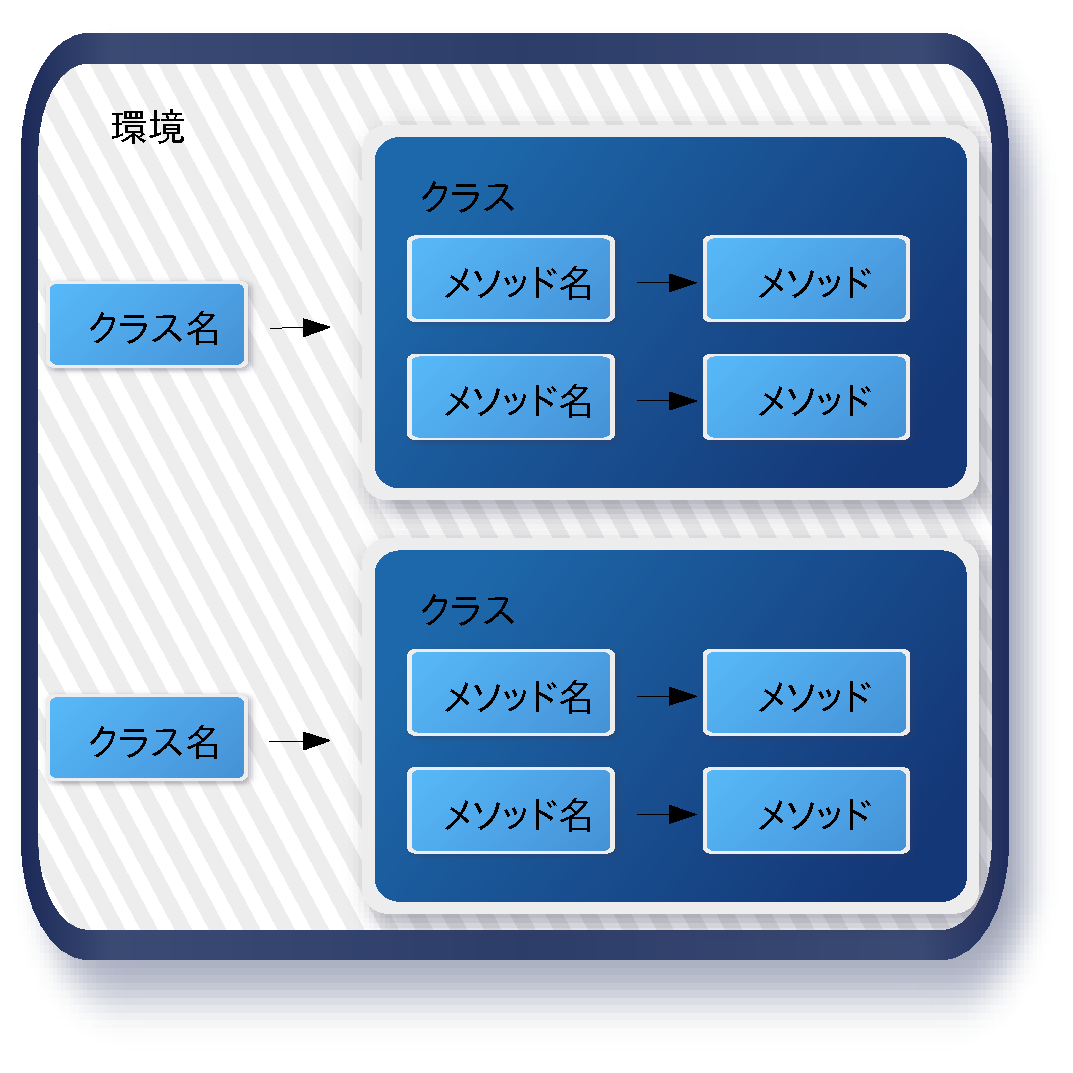
\includegraphics[width=7cm]{fig/classes-crop.pdf}
\caption{クラスにメソッドを格納するモデル}
\label{fig:classes}
\end{figure}

\begin{figure}
\centering
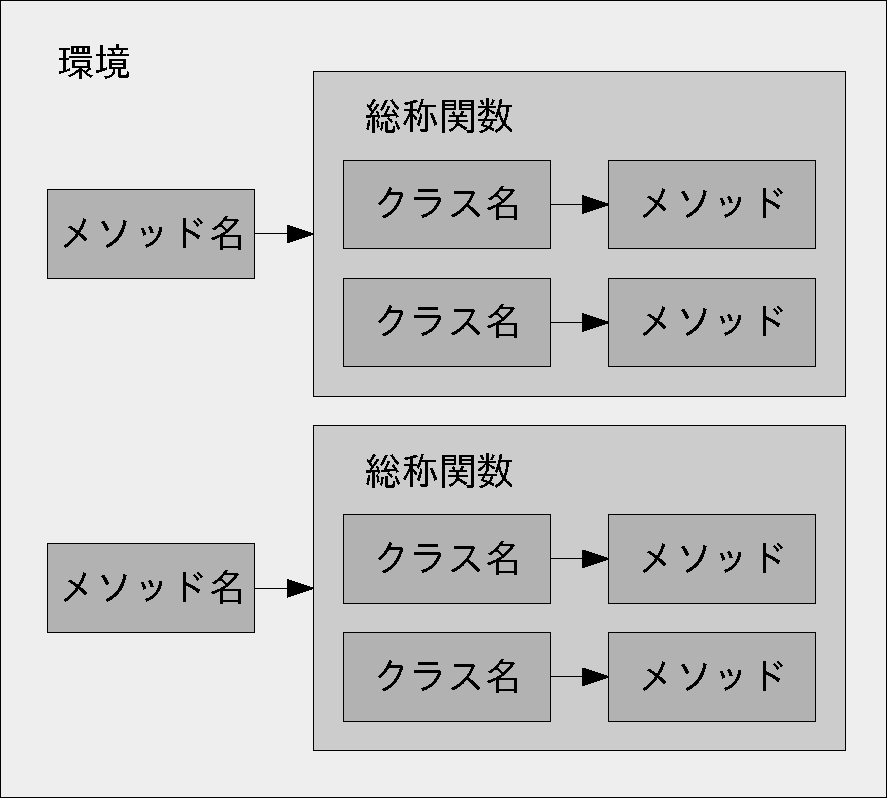
\includegraphics[width=7cm]{fig/generic-functions-crop.pdf}
\caption{総称関数にメソッドを格納するモデル}
\label{fig:generic-functions}
\end{figure}

\begin{figure}
\centering
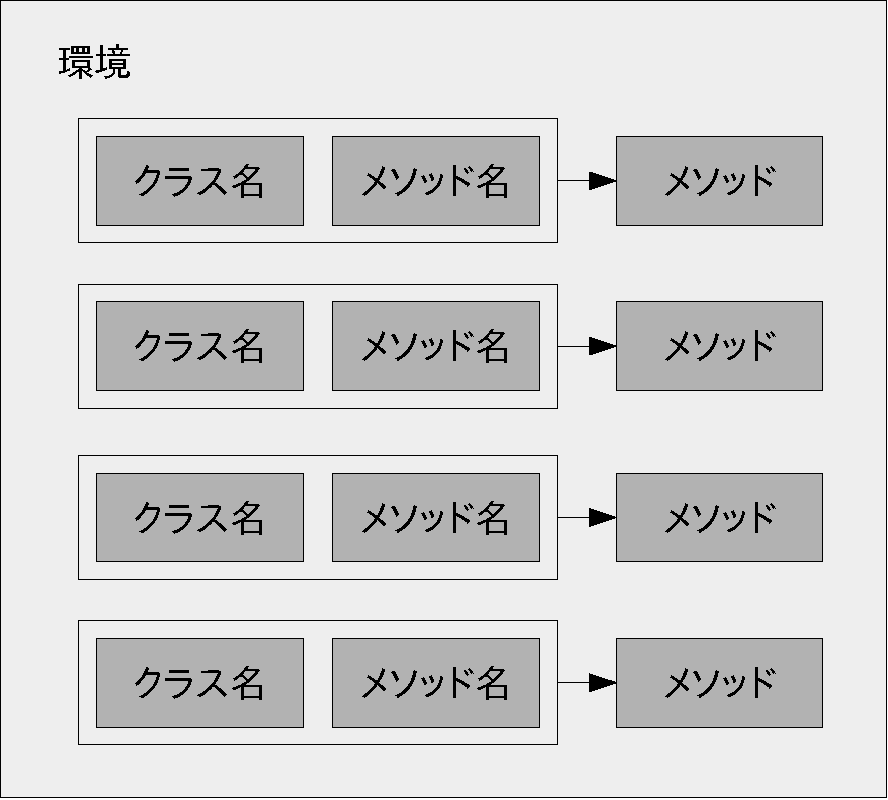
\includegraphics[width=7cm]{fig/environment-crop.pdf}
\caption{環境にメソッドを直接格納するモデル}
\label{fig:environment}
\end{figure}

\section{提案するオブジェクトシステム}

従来のオブジェクトシステムの分類先である2つのモデルは,どちらもクラス名とメソッド名が決まれば
メソッドが一意に定まるという特徴を持つ.
また,環境という辞書の中にクラスあるいは総称関数という辞書が入れ子になっている構造も
共通している.

提案するオブジェクトシステムはこのようなクラスや総称関数による入れ子構造を廃し,
\textbf{環境にメソッドを直接格納するモデル}を採用する(図\ref{fig:environment}).
ここで環境は\textbf{クラス名とメソッド名の組}をキーとしてメソッドを格納する辞書である.

このモデルの特徴は,メソッドの格納方式が一般的な変数の格納方式と類似していることである.
メソッドがクラス名とメソッド名の組をキーとして環境に格納されるのに対し,変数は変数名を
キーとして環境に格納される.

これはすなわち,「変数名」を「クラス名とメソッド名の組」に置き換えることで,
\textbf{変数に対して行えるあらゆる操作がメソッドに対しても行えるようになる}ということである.
具体的には,ブロック単位でのスコープの制御やシャドーイング,モジュールからのエクスポート・
インポート,仮引数やパターンマッチングのパターンとしての指定などが挙げられる.
\ref{sec:implementation}節では提案するオブジェクトシステムを搭載した独自の
プログラミング言語Suzuを用いて,この特徴を生かした実際のプログラム例を示す.

\section{実装:プログラミング言語Suzu}
\label{sec:implementation}

提案する手法の有用性を実証するため,独自に設計したプログラミング言語Suzuを実装した.
Suzuは,クラス・コンストラクタ・セッター・ゲッター・メソッドといったオブジェクト指向プログラミングにおける
種々の概念に加え,トレイトやユーザ定義演算子,ラベル付き引数,ブロック付き関数呼び出し,
限定継続などの機構を搭載している.これらの機構が,オブジェクトシステムの利点を生かし,
PEGパーザコンビネータのようなドメイン特化言語を作成する際に有用であることを示す.

\subsection{シンタックス}

\begin{quote}
\small
\begin{verbatim}
class <class> = <ctor>:
  [mutable] <field>*
end
\end{verbatim}
\end{quote}

\subsection{セマンティクス}

\subsection{プログラム例}

\subsubsection{PEGパーザコンビネータ}

\section{比較}

クラスにメソッドを格納するオブジェクトシステムの拡張機構について,本提案がより自然な形で同等
もしくはそれ以上の機能を提供していることを示す.

クラスにメソッドを格納する方式のオブジェクトシステムにおいて提案するオブジェクトシステムに似た
柔軟性を実現するための既存の機構であるRefinementsやClassbox,MethodShelters,
拡張メソッド等との関連や,概念的に類似したHaskellの型クラスおよびMixJuiceとの関連についても
議論する.

\section{今後の課題}

\subsection{継承機構}

Suzuは継承機構を持たず,Traitsによって実装の再利用を行う.
継承機構を持たないことによって生じる不都合については今後検討していく必要がある.

もしSuzuに継承機構を追加するとしてもそれほど複雑にはならない.
オブジェクトは1つのクラス名しか持たないという現在の仕様を拡張し,複数のクラス名を
先頭からメソッド解決順序に基づき並べたリストで持つようにすればよい.
メソッド呼び出しの際はオブジェクトが持つリストの先頭から順にクラス名を取り出し,
メソッド名との組を作りこれをキーとして環境からメソッドの探索を行う(TODO:図の挿入?).

単一継承に制限する場合,クラス名のリストは先頭が継承ツリーの最下位クラス,
末尾が最上位クラスとなる.
多重継承を許す場合,C3線形化\cite{Barrett:1996:MSL:236337.236343}等を用いて
適切な順序で並べたクラス名のリストを生成する必要がある.

\subsection{多重ディスパッチ}
\label{sec:multiple-dispatch}

\ref{sec:generic-finctions}節で示した総称関数にメソッドを格納するモデルは,
CLOSがサポートする多重ディスパッチに対応していない.
モデルを多重ディスパッチに対応させるには,総称関数を単なる辞書ではなくある種のデータベース
としてとらえる必要がある.
データベースは各引数から集めた複数のクラス名を受け取って,その組み合わせにマッチするメソッドを
検索し返す.

Suzuは多重ディスパッチに対応していないが,このモデルを応用し対応させることが可能である.
すなわち環境をある種のデータベースとしてとらえ,複数のクラス名と1つのメソッド名を受け取って
その組み合わせにマッチするメソッドを検索し返す.

つまり,1つのクラス名と1つのメソッド名からメソッドが決まるのが単一ディスパッチ,
複数のクラス名と1つのメソッド名からメソッドが決まるのが多重ディスパッチであると言える.
ここで自然と,1つのクラス名と複数のメソッド名または複数のクラス名と複数のメソッド名から
メソッドが決まるオブジェクトシステムというのも思い浮かぶ.
これらは既存のオブジェクトシステムにない概念であり,考察の余地がある.

\subsection{メソッド呼び出しの高速化}

(TODO:マンデルブロ集合の計算にかかった時間を記載?)

Suzuのオブジェクトシステムには,メソッド呼び出しの一般的な高速化手法がそのまま適用できない
ことがある.
例として,動的型付け言語においてよく使用されるキャッシュ法\cite{Onodera:1997}のうち,
メソッドキャッシュとインラインキャッシュについて検討する.

メソッドキャッシュはグローバルな空間に1つだけ用意されるキャッシュである.
同じクラス名とメソッド名の組に対してメソッド呼び出しが行われた場合,キャッシュ内容に基づき
メソッドを返すため探索を行わなくて済む.
Suzuはメソッドのローカル定義を許すため,同じクラス名とメソッド名の組であっても
呼び出す場所によってメソッドの探索結果が異なる.
よって,グローバルな空間に1つだけキャッシュを用意するメソッドキャッシュは適用できない.

インラインキャッシュはメソッド呼び出しを行う仮想マシン命令の内部に用意されるキャッシュである.
こちらは呼び出し位置に対応してキャッシュが存在するのでメソッドのローカル定義にも対応できる.
ただし,Suzuは仮引数としてメソッドを指定することができるため関数呼び出しのたびにメソッドの
内容が異なることもあり,メソッドの値を直接キャッシュしてはならない.
環境においてメソッドが格納場所を固定し,格納場所を指すインデックスをキャッシュする必要がある.

\section{結論}

従来のオブジェクトシステムはクラスにメソッドを格納するモデルと総称関数にメソッドを格納する
モデルとに分類されたが,そのどちらにも属さない,環境にメソッドを直接格納するモデルを持つ
オブジェクトシステムを提案した.

特徴は変数に対して行えるあらゆる操作がメソッドに対しても行えるようになることである.
プログラミング言語Suzuを用いてこの特徴を生かした言語内DSLを作成し,提案する
オブジェクトシステムの有用性を示した.

オブジェクト指向プログラミングにおける既存の概念の整理にも役立った.
今後はより実用性を意識した拡張や効率的な実装について考えていくことが課題である.

%\begin{acknowledgment}
%謝辞が必要であれば,ここに書く.
%\end{acknowledgment}

% BibTeX を使用する場合 %%%%%%%%%%%%%%%%%%%%%%%%%%%%%%%%%
\bibliographystyle{ipsjsort}
\bibliography{thesis}

% BibTeX を使用しない場合
%\begin{thebibliography}{9}
%\bibitem{latex} 奥村晴彦, 黒木裕介: \textbf{LaTeX2e美文書作成入門}. 技術評論社, 2013.
%\end{thebibliography}

\end{document}
